\documentclass[master=emitm,masteroption=bc,oneside]{kulemt}
\DisemulatePackage{setspace}
\usepackage{setspace}
\usepackage{pdfpages}
\usepackage{amsmath}
\usepackage{pgf,tikz}
\usetikzlibrary{positioning, arrows.meta, matrix, backgrounds, shapes.misc}
\usetikzlibrary{calc,arrows}

\makeatletter

%%%%%%%%%%%%%%%%%%% Begin add-int-rnd %%%%%%%%%%%%%%%
% Data Flip Flip (DFF) shape
\pgfdeclareshape{dff}{
	% The 'minimum width' and 'minimum height' keys, not the content, determine
	% the size
	\savedanchor\northeast{%
		\pgfmathsetlength\pgf@x{\pgfshapeminwidth}%
		\pgfmathsetlength\pgf@y{\pgfshapeminheight}%
		\pgf@x=0.5\pgf@x
		\pgf@y=0.5\pgf@y
	}
	% This is redundant, but makes some things easier:
	\savedanchor\southwest{%
		\pgfmathsetlength\pgf@x{\pgfshapeminwidth}%
		\pgfmathsetlength\pgf@y{\pgfshapeminheight}%
		\pgf@x=-0.5\pgf@x
		\pgf@y=-0.5\pgf@y
	}
	% Inherit from rectangle
	\inheritanchorborder[from=rectangle]
	
	% Define same anchor a normal rectangle has
	\anchor{center}{\pgfpointorigin}
	\anchor{north}{\northeast \pgf@x=0pt}
	\anchor{east}{\northeast \pgf@y=0pt}
	\anchor{south}{\southwest \pgf@x=0pt}
	\anchor{west}{\southwest \pgf@y=0pt}
	\anchor{north east}{\northeast}
	\anchor{north west}{\northeast \pgf@x=-\pgf@x}
	\anchor{south west}{\southwest}
	\anchor{south east}{\southwest \pgf@x=-\pgf@x}
	\anchor{text}{
		\pgfpointorigin
		\advance\pgf@x by -.5\wd\pgfnodeparttextbox%
		\advance\pgf@y by -.5\ht\pgfnodeparttextbox%
		\advance\pgf@y by +.5\dp\pgfnodeparttextbox%
	}
	
	% Define anchors for signal ports
	\anchor{D}{
		\pgf@process{\northeast}%
		\pgf@x=-1\pgf@x%
		\pgf@y=.5\pgf@y%
	}
	\anchor{CLK}{
		\pgf@process{\northeast}%
		\pgf@x=-1\pgf@x%
		\pgf@y=-.66666\pgf@y%
	}
	\anchor{CE}{
		\pgf@process{\northeast}%
		\pgf@x=-1\pgf@x%
		\pgf@y=-0.33333\pgf@y%
	}
	\anchor{Q}{
		\pgf@process{\northeast}%
		\pgf@y=.5\pgf@y%
	}
	\anchor{Qn}{
		\pgf@process{\northeast}%
		\pgf@y=-.5\pgf@y%
	}
	\anchor{R}{
		\pgf@process{\northeast}%
		\pgf@x=0pt%
	}
	\anchor{S}{
		\pgf@process{\northeast}%
		\pgf@x=0pt%
		\pgf@y=-\pgf@y%
	}
	% Draw the rectangle box and the port labels
	\backgroundpath{
		% Rectangle box
		\pgfpathrectanglecorners{\southwest}{\northeast}
		% Angle (>) for clock input
		\pgf@anchor@dff@CLK
		\pgf@xa=\pgf@x \pgf@ya=\pgf@y
		\pgf@xb=\pgf@x \pgf@yb=\pgf@y
		\pgf@xc=\pgf@x \pgf@yc=\pgf@y
		\pgfmathsetlength\pgf@x{1.6ex} % size depends on font size
		\advance\pgf@ya by \pgf@x
		\advance\pgf@xb by \pgf@x
		\advance\pgf@yc by -\pgf@x
		\pgfpathmoveto{\pgfpoint{\pgf@xa}{\pgf@ya}}
		%		\pgfpathlineto{\pgfpoint{\pgf@xb}{\pgf@yb}}
		%		\pgfpathlineto{\pgfpoint{\pgf@xc}{\pgf@yc}}
		\pgfclosepath
		
		% Draw port labels
		\begingroup
		\tikzset{flip flop/port labels} % Use font from this style
		\tikz@textfont
		\endgroup
	}
}

%%%%%%%%%%%%%%%%%%% End add-int-rnd %%%%%%%%%%%%%%%

% Key to add font macros to the current font
\tikzset{add font/.code={\expandafter\def\expandafter\tikz@textfont\expandafter{\tikz@textfont#1}}} 

% Define default style for this node
\tikzset{flip flop/port labels/.style={font=\sffamily\scriptsize}}
\tikzset{every dff node/.style={draw,minimum width=1.0cm,minimum 
		height=0.5cm,very thick,inner sep=1mm,outer sep=0pt,cap=round,add 
		font=\sffamily}}
%\usepackage{kulemtx}
%\headstyles{kulemtman}
%\kulemtmanToC


\setup{title={Metrics of Operating System Security Components in Virtual Environments},
  author={Oliver Jessl},
  promotor={Prof. Dr.-Ing. Clemens Martin},
  assessor={Prof. Dr.-Ing. habil. Dennis Pfisterer},
  assistant={}}
% The following \setup may be removed entirely if no filing card is wanted
\setup{filingcard,
  translatedtitle=,
  udc=621.3,
  shortabstract={Here comes a very short abstract, containing no more than 500
    words. \LaTeX\ commands can be used here. Blank lines (or the command
    \texttt{\string\pa r}) are not allowed!
    \endgraf \lipsum[2]}}
% Uncomment the next line for generating the cover page
%\setup{coverpageonly}
% Uncomment the next \setup to generate only the first pages (e.g., if you
% are a Word user.
%\setup{frontpagesonly}

\setlrmarginsandblock{3cm}{3cm}{*}
\setulmarginsandblock{3cm}{3cm}{*}
\checkandfixthelayout

% Choose the main text font (e.g., Latin Modern)
\setup{font=times}

% If you want to include other LaTeX packages, do it here. 

% Finally the hyperref package is used for pdf files.
% This can be commented out for printed versions.
\usepackage[pdfusetitle,colorlinks,plainpages=false]{hyperref}

%%%%%%%
% The lipsum package is used to generate random text.
% You never need this in a real master's thesis text!
\IfFileExists{lipsum.sty}%
 {\usepackage{lipsum}\setlipsumdefault{11-13}}%
 {\newcommand{\lipsum}[1][11-13]{\par And some text: lipsum ##1.\par}}
%%%%%%%



%\onehalfspacing
\onehalfspacing

%\includeonly{chap-n}
\begin{document}



\begin{preface}
  I would like to thank everybody who kept me busy the last year,
  especially my promoter and my assistants. I would also like to thank the
  jury for reading the text. My sincere gratitude also goes to my wive and
  the rest of my family.
\end{preface}



\tableofcontents*

\begin{abstract}
  The \texttt{abstract} environment contains a more extensive overview of
  the work. But it should be limited to one page.

  \lipsum[1]
\end{abstract}

% A list of figures and tables is optional
%\listoffigures
%\listoftables
% If you only have a few figures and tables you can use the following instead
\listoffiguresandtables
% The list of symbols is also optional.
% This list must be created manually, e.g., as follows:
\chapter{List of Abbreviations and Symbols}
\section*{Abbreviations}
\begin{flushleft}
  \renewcommand{\arraystretch}{1.1}
  \begin{tabularx}{\textwidth}{@{}p{12mm}X@{}}
    ASLR  & Address Space Randomization Layout \\  	
    GRI   & Get Random Int (Random Number Generator)\\
	GRL	  & Get Random Long (Random Number Generator)\\
    NIST  & National Institute of Standards and Technology \\
    PRNG  & Pseudo Random Number Generator \\    
    TRNG  & True Random Number Generator \\        
    VM	  & Virtual Machine \\
  \end{tabularx}
\end{flushleft}
\section*{Symbols}
\begin{flushleft}
  \renewcommand{\arraystretch}{1.1}
  \begin{tabularx}{\textwidth}{@{}p{12mm}X@{}}
    42    & ``The Answer to the Ultimate Question of Life, the Universe,
            and Everything'' according to \cite{h2g2} \\
    $c$   & Speed of light \\
    $E$   & Energy \\
    $m$   & Mass \\
    $\pi$ & The number pi \\
  \end{tabularx}
\end{flushleft}


	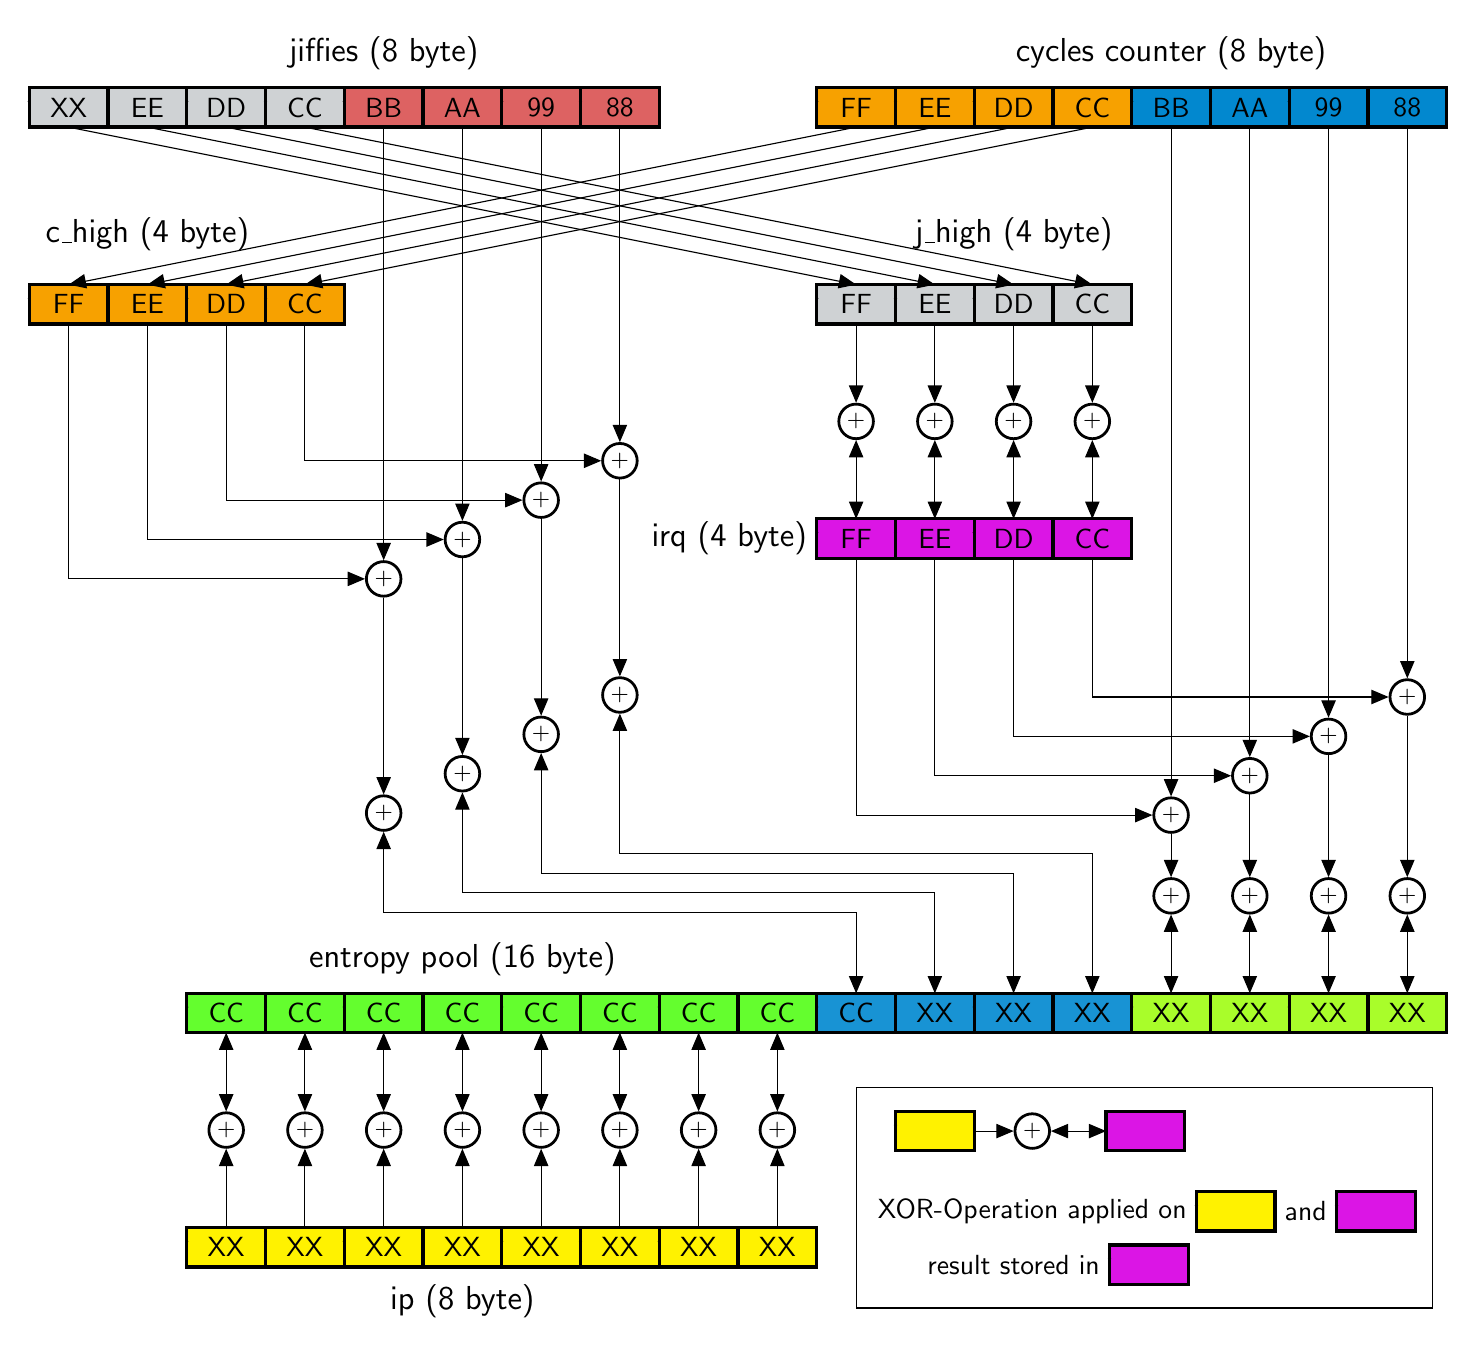
\begin{tikzpicture}[font=\sffamily,>=triangle 45]
	\tikzstyle{sum} = [draw, shape=circle, node distance=1.5cm, line width=1pt, minimum width=1.25em]	
	%\Huge
	\def\N{7}  % Number of Flip-Flops minus one
	\def\BW{1.8} % Byte Width
	
	% colors
	\definecolor{cjh}{HTML}{CFD2D4}
	\definecolor{cjl}{HTML}{DD6262}
	\definecolor{cch}{HTML}{F7A100}
	\definecolor{ccl}{HTML}{0288CF}
	\definecolor{cep32}{HTML}{64FE2E}
	\definecolor{cep1}{HTML}{1893D4}
	\definecolor{cep0}{HTML}{A9FD2A}
	\definecolor{cirq}{HTML}{DB15E5}
	\definecolor{cip}{HTML}{FFF200}
	
	% jiffies
	\node [shape=dff,fill=cjh] (jiff7) at ($ 1.0*(0,0) $) {XX};
	\node [shape=dff,fill=cjh] (jiff6) at ($ 1.0*(1,0) $) {EE};
	\node [shape=dff,fill=cjh] (jiff5) at ($ 1.0*(2,0) $) {DD};
	\node [shape=dff,fill=cjh] (jiff4) at ($ 1.0*(3,0) $) {CC};			
	\node [shape=dff,fill=cjl] (jiff3) at ($ 1.0*(4,0) $) {BB};
	\node [shape=dff,fill=cjl] (jiff2) at ($ 1.0*(5,0) $) {AA};
	\node [shape=dff,fill=cjl] (jiff1) at ($ 1.0*(6,0) $) {99};
	\node [shape=dff,fill=cjl] (jiff0) at ($ 1.0*(7,0) $) {88};	
	\node[above=1mm of jiff3] (ljiffies) {\large jiffies (8 byte)};		
	
	% jiffies low XOR c_high - XOR nodes
	\node [sum, below=4.0cm of jiff0, draw] (xjlch0) {};
	\node [sum, below=4.5cm of jiff1, draw] (xjlch1) {};	
	\node [sum, below=5.0cm of jiff2, draw] (xjlch2) {};
	\node [sum, below=5.5cm of jiff3, draw] (xjlch3) {};	
	\node at (xjlch0) (plus) {{\footnotesize$+$}};
	\node at (xjlch1) (plus) {{\footnotesize$+$}};	
	\node at (xjlch2) (plus) {{\footnotesize$+$}};
	\node at (xjlch3) (plus) {{\footnotesize$+$}};
	
	% cycles
	\node [shape=dff,fill=cch] (cycl7) at ($ 1.0*(10,0) $) {FF};
	\node [shape=dff,fill=cch] (cycl6) at ($ 1.0*(11,0) $) {EE};
	\node [shape=dff,fill=cch] (cycl5) at ($ 1.0*(12,0) $) {DD};
	\node [shape=dff,fill=cch] (cycl4) at ($ 1.0*(13,0) $) {CC};			
	\node [shape=dff,fill=ccl] (cycl3) at ($ 1.0*(14,0) $) {BB};
	\node [shape=dff,fill=ccl] (cycl2) at ($ 1.0*(15,0) $) {AA};
	\node [shape=dff,fill=ccl] (cycl1) at ($ 1.0*(16,0) $) {99};
	\node [shape=dff,fill=ccl] (cycl0) at ($ 1.0*(17,0) $) {88};
	\node[above=1mm of cycl3] (lcycles) {\large cycles counter (8 byte)};	
	
	%c_high
	\node [shape=dff,fill=cch, below=2cm of jiff7, draw] (chigh3) {FF};
	\node [shape=dff,fill=cch, below=2cm of jiff6, draw] (chigh2) {EE};
	\node [shape=dff,fill=cch, below=2cm of jiff5, draw] (chigh1) {DD};
	\node [shape=dff,fill=cch, below=2cm of jiff4, draw] (chigh0) {CC};
	\node[above=3mm of chigh2] (lchigh) {\large c\_high (4 byte)};			
	
	%j_high
	\node [shape=dff,fill=cjh, below=2cm of cycl7, draw] (jiffh3) {FF};
	\node [shape=dff,fill=cjh, below=2cm of cycl6, draw] (jiffh2) {EE};
	\node [shape=dff,fill=cjh, below=2cm of cycl5, draw] (jiffh1) {DD};
	\node [shape=dff,fill=cjh, below=2cm of cycl4, draw] (jiffh0) {CC};
	\node[above=3mm of jiffh1] (ljhigh) {\large j\_high (4 byte)};			
	
	% jiffies high XOR irq - XOR nodes
	\node [sum, below=1.0cm of jiffh3, draw] (xjhi3) {};	
	\node at (xjhi3) (plus) {{\footnotesize$+$}};
	\node [sum, below=1.0cm of jiffh2, draw] (xjhi2) {};	
	\node at (xjhi2) (plus) {{\footnotesize$+$}};
	\node [sum, below=1.0cm of jiffh1, draw] (xjhi1) {};	
	\node at (xjhi1) (plus) {{\footnotesize$+$}};
	\node [sum, below=1.0cm of jiffh0, draw] (xjhi0) {};	
	\node at (xjhi0) (plus) {{\footnotesize$+$}};
	
	%irq
	\node [shape=dff,fill=cirq, below=1cm of xjhi3, draw] (irq3) {FF};
	\node [shape=dff,fill=cirq, below=1cm of xjhi2, draw] (irq2) {EE};
	\node [shape=dff,fill=cirq, below=1cm of xjhi1, draw] (irq1) {DD};
	\node [shape=dff,fill=cirq, below=1cm of xjhi0, draw] (irq0) {CC};
	\node[left=0mm of irq3] (lirq) {\large irq (4 byte)};	
	
	% cycles low XOR irq - XOR nodes
	\node [sum, below=8.5cm of cycl3, draw] (xcli3) {};
	\node [sum, below=8.0cm of cycl2, draw] (xcli2) {};	
	\node [sum, below=7.5cm of cycl1, draw] (xcli1) {};		
	\node [sum, below=7.0cm of cycl0, draw] (xcli0) {};			
	\node at (xcli3) (plus) {{\footnotesize$+$}};
	\node at (xcli2) (plus) {{\footnotesize$+$}};	
	\node at (xcli1) (plus) {{\footnotesize$+$}};
	\node at (xcli0) (plus) {{\footnotesize$+$}};	
	
	% entropy pool	
	\node [shape=dff,fill=cep32, below=11cm of jiff5, draw] (entp15) {CC};		
	\node [shape=dff,fill=cep32, below=11cm of jiff4, draw] (entp14) {CC};
	\node [shape=dff,fill=cep32, below=11cm of jiff3, draw] (entp13) {CC};
	\node [shape=dff,fill=cep32, below=11cm of jiff2, draw] (entp12) {CC};
	\node [shape=dff,fill=cep32, below=11cm of jiff1, draw] (entp11) {CC};
	\node [shape=dff,fill=cep32, below=11cm of jiff0, draw] (entp10) {CC};
	\node [shape=dff,fill=cep32, right=0cm of entp10, draw] (entp9) {CC};	
	\node [shape=dff,fill=cep32, right=0cm of entp9, draw] (entp8) {CC};
	\node [shape=dff,fill=cep1, right=0cm of entp8, draw] (entp7) {CC};
	\node [shape=dff,fill=cep1, below=11cm of cycl6, draw] (entp6) {XX};	
	\node [shape=dff,fill=cep1, below=11cm of cycl5, draw] (entp5) {XX};	
	\node [shape=dff,fill=cep1, below=11cm of cycl4, draw] (entp4) {XX};	
	\node [shape=dff,fill=cep0, below=11cm of cycl3, draw] (entp3) {XX};	
	\node [shape=dff,fill=cep0, below=11cm of cycl2, draw] (entp2) {XX};	
	\node [shape=dff,fill=cep0, below=11cm of cycl1, draw] (entp1) {XX};	
	\node [shape=dff,fill=cep0, below=11cm of cycl0, draw] (entp0) {XX};	
	\node[above=1mm of entp12] (lentp) {\large entropy pool (16 byte)};	
	
	%% XOR entp
	% ch / jl 
	\node [sum, below=2.5cm of xjlch3, draw] (xentp7) {};	
	\node at (xentp7) (plus) {{\footnotesize$+$}};
	\node [sum, below=2.5cm of xjlch2, draw] (xentp6) {};	
	\node at (xentp6) (plus) {{\footnotesize$+$}};
	\node [sum, below=2.5cm of xjlch1, draw] (xentp5) {};	
	\node at (xentp5) (plus) {{\footnotesize$+$}};
	\node [sum, below=2.5cm of xjlch0, draw] (xentp4) {};	
	\node at (xentp4) (plus) {{\footnotesize$+$}};									
	% irq/cycl 
	\node [sum, above=1.0cm of entp3, draw] (xentp3) {};	
	\node at (xentp3) (plus) {{\footnotesize$+$}};
	\node [sum, above=1.0cm of entp2, draw] (xentp2) {};	
	\node at (xentp2) (plus) {{\footnotesize$+$}};
	\node [sum, above=1.0cm of entp1, draw] (xentp1) {};	
	\node at (xentp1) (plus) {{\footnotesize$+$}};
	\node [sum, above=1.0cm of entp0, draw] (xentp0) {};	
	\node at (xentp0) (plus) {{\footnotesize$+$}};		
	% ip
	\node [sum, below=1.0cm of entp15, draw] (xentp15) {};	
	\node at (xentp15) (plus) {{\footnotesize$+$}};
	\node [sum, below=1.0cm of entp14, draw] (xentp14) {};	
	\node at (xentp14) (plus) {{\footnotesize$+$}};
	\node [sum, below=1.0cm of entp13, draw] (xentp13) {};	
	\node at (xentp13) (plus) {{\footnotesize$+$}};
	\node [sum, below=1.0cm of entp12, draw] (xentp12) {};	
	\node at (xentp12) (plus) {{\footnotesize$+$}};		
	\node [sum, below=1.0cm of entp11, draw] (xentp11) {};	
	\node at (xentp11) (plus) {{\footnotesize$+$}};
	\node [sum, below=1.0cm of entp10, draw] (xentp10) {};	
	\node at (xentp10) (plus) {{\footnotesize$+$}};
	\node [sum, below=1.0cm of entp9, draw] (xentp9) {};	
	\node at (xentp9) (plus) {{\footnotesize$+$}};
	\node [sum, below=1.0cm of entp8, draw] (xentp8) {};	
	\node at (xentp8) (plus) {{\footnotesize$+$}};	
	
	\node [shape=dff,fill=cip, below=1cm of xentp15, draw] (ip7) {XX};	
	\node [shape=dff,fill=cip, below=1cm of xentp14, draw] (ip6) {XX};
	\node [shape=dff,fill=cip, below=1cm of xentp13, draw] (ip5) {XX};
	\node [shape=dff,fill=cip, below=1cm of xentp12, draw] (ip4) {XX};
	\node [shape=dff,fill=cip, below=1cm of xentp11, draw] (ip3) {XX};
	\node [shape=dff,fill=cip, below=1cm of xentp10, draw] (ip2) {XX};
	\node [shape=dff,fill=cip, below=1cm of xentp9, draw] (ip1) {XX};
	\node [shape=dff,fill=cip, below=1cm of xentp8, draw] (ip0) {XX};
	\node[below=1mm of ip4] (lip) {\large ip (8 byte)};	
	
	%%%%%% LINES >>
	
	% jiffies  -> c_low - lines
	\draw [->] (jiff3.south) -- (xjlch3.north);
	\draw [->] (jiff2.south) -- (xjlch2.north);	
	\draw [->] (jiff1.south) -- (xjlch1.north);		
	\draw [->] (jiff0.south) -- (xjlch0.north);		
	
	% c_high -> xjlch
	\draw [->] (chigh3.south)|- (xjlch3.west);
	\draw [->] (chigh2.south)|- (xjlch2.west);
	\draw [->] (chigh1.south)|- (xjlch1.west);
	\draw [->] (chigh0.south)|- (xjlch0.west);			
	
	% jiffies high -> j_high
	\draw [->] (jiff7.south) -- (jiffh3.north);
	\draw [->] (jiff6.south) -- (jiffh2.north);	
	\draw [->] (jiff5.south) -- (jiffh1.north);		
	\draw [->] (jiff4.south) -- (jiffh0.north);		
	
	% cycles_high -> c_high
	\draw [->] (cycl7.south) -- (chigh3.north);
	\draw [->] (cycl6.south) -- (chigh2.north);	
	\draw [->] (cycl5.south) -- (chigh1.north);		
	\draw [->] (cycl4.south) -- (chigh0.north);		
	
	% cycles_low -> c_high
	\draw [->] (cycl3.south) -- (xcli3.north);
	\draw [->] (cycl2.south) -- (xcli2.north);	
	\draw [->] (cycl1.south) -- (xcli1.north);		
	\draw [->] (cycl0.south) -- (xcli0.north);	
	
	% jiffies high -> j_high
	\draw [->] (jiffh3.south) -- (xjhi3.north);
	\draw [->] (jiffh2.south) -- (xjhi2.north);	
	\draw [->] (jiffh1.south) -- (xjhi1.north);		
	\draw [->] (jiffh0.south) -- (xjhi0.north);
	
	% xjhi -> irq
	\draw [<->] (xjhi3.south) -- (irq3.north);
	\draw [<->] (xjhi2.south) -- (irq2.north);	
	\draw [<->] (xjhi1.south) -- (irq1.north);		
	\draw [<->] (xjhi0.south) -- (irq0.north);
	
	% xjlch -> xentp
	\draw [->] (xjlch3.south) -- (xentp7.north);
	\draw [->] (xjlch2.south) -- (xentp6.north);	
	\draw [->] (xjlch1.south) -- (xentp5.north);		
	\draw [->] (xjlch0.south) -- (xentp4.north);
	
	% irq -> xcli
	\draw [->] (irq3.south) |- (xcli3.west);
	\draw [->] (irq2.south) |- (xcli2.west);	
	\draw [->] (irq1.south) |- (xcli1.west);		
	\draw [->] (irq0.south) |- (xcli0.west);
	
	% xentp -> entp
	\draw [<->] (xentp7.south) |- ($(entp7.north)!1/2!(entp7.north |- xentp7.south)$) coordinate (C1) -| (entp7.north);			
	\draw [<->] (xentp6.south) |- ($(entp6.north)!1/2!(entp6.north |- xentp6.south)$) coordinate (C2) -| (entp6.north);		
	\draw [<->] (xentp5.south) |- ($(entp5.north)!1/2!(entp5.north |- xentp5.south)$) coordinate (C3) -| (entp5.north);				
	\draw [<->] (xentp4.south) |- ($(entp4.north)!1/2!(entp4.north |- xentp4.south)$) coordinate (C4) -| (entp4.north);	
	
	% xcli -> xentp
	\draw [->] (xcli3.south) -- (xentp3.north);
	\draw [->] (xcli2.south) -- (xentp2.north);	
	\draw [->] (xcli1.south) -- (xentp1.north);		
	\draw [->] (xcli0.south) -- (xentp0.north);	
	
	% xcli -> xentp
	\draw [<->] (xentp3.south) -- (entp3.north);
	\draw [<->] (xentp2.south) -- (entp2.north);	
	\draw [<->] (xentp1.south) -- (entp1.north);		
	\draw [<->] (xentp0.south) -- (entp0.north);
	
	% xentp -> entp
	\draw [<->] (xentp15.north) -- (entp15.south);
	\draw [<->] (xentp14.north) -- (entp14.south);
	\draw [<->] (xentp13.north) -- (entp13.south);
	\draw [<->] (xentp12.north) -- (entp12.south);
	\draw [<->] (xentp11.north) -- (entp11.south);
	\draw [<->] (xentp10.north) -- (entp10.south);
	\draw [<->] (xentp9.north) -- (entp9.south);
	\draw [<->] (xentp8.north) -- (entp8.south);
	
	% ip -> xentp
	\draw [->] (ip7.north) -- (xentp15.south);
	\draw [->] (ip6.north) -- (xentp14.south);
	\draw [->] (ip5.north) -- (xentp13.south);
	\draw [->] (ip4.north) -- (xentp12.south);
	\draw [->] (ip3.north) -- (xentp11.south);
	\draw [->] (ip2.north) -- (xentp10.south);
	\draw [->] (ip1.north) -- (xentp9.south);
	\draw [->] (ip0.north) -- (xentp8.south);
	
	%%%%%% Legende 
	\begin{scope}
	\node [shape=dff,fill=cip, below=10mm of entp6, draw] (f8) {};
	\node [sum, right=5mm of f8, draw] (xf8) {};	
	\node at (xf8) (plus) {{\footnotesize$+$}};	
	\node [shape=dff,fill=cirq, right=7mm of xf8, draw] (c3) {};
	\draw [->] (f8.east) -- (xf8.west);
	\draw [<->] (xf8.east) -- (c3.west);
	\node[black, below=5mm of xf8, align=left] (lf81) {XOR-Operation applied on};	
	\node [shape=dff,fill=cip, right=0mm of lf81, draw] (rf8) {};
	\node[black, right=0mm of rf8, align=left] (lf82) {and};	
	\node [shape=dff,fill=cirq, right=0mm of lf82, draw] (yf8) {};
	\node[black, below=27mm of entp5, align=left] (lf83) {result stored in};	
	\node [shape=dff,fill=cirq, right=0mm of lf83, draw] (zf8) {};	
	\draw[black] ([xshift=-5mm, yshift=3mm ]f8.north west) rectangle ([xshift=31mm, yshift=-3mm]zf8.south east);	
	\end{scope}	
	\end{tikzpicture}

% Now comes the main text
\mainmatter

\chapter{Introduction}
\label{cha:intro}
\section{Motivation}
Operating systems implement a variety of security components which depend significantly on the entropy of random numbers. In general, those random numbers can be provided by operating system internal or external providers, so called Random Number Generators (RNG). Typical external providers are hardware devices, able to deviate random numbers from radioactive decay, atmospheric or thermal noise, photoelectric effects etc. Since those numbers are assumed to provide a high level of entropy i.e. random numbers of high quality, they are also referred as True Random Number Generators (TRNG). Contrary, RNGs implemented as part of an operating system, the lack of comparable stochastic processes and hence are labeled as Pseudo Random Number Generator (PRNG). To compensate this lack, PRGN implementations need to fall back on alternative sources, able to provide information with a certain degree of entropy. Common approaches of operating systems usually adopt information from external sources, f.e. user input like keyboard events or mouse coordinates. Beside further external input like network traffic, system internal individual information like serial numbers of hardware devices, MAC addresses or the occurrence of hardware interrupts is used to gain an entropy pool of pseudo random numbers. Consequently, the process of generating random numbers by an operating system PRNG is influenced by the way the system interacts with its environment i.e. how it is set up. This aspect should be considered when applying server operating systems as virtual machines i.e. in virtual environments. \\~\\
Virtualization of operating systems has increased continuously over the recent years and layed the foundations for new resource management concepts and business models like f.e. cloud hosting. Regarding server virtualization, many organizations exceed rates of 75\% \cite{gartnervmmarket}. By executing an operating system as a virtual machine, improvements in several areas, like scalability and more efficient utilization of hardware resources, backup \& disaster recovery strategy, accelerated provision of new system instances etc. can be achieved. Depending on the applied technology, such virtual machines can be setup up on basis of operating system setup images which are targeted for installation directly on hardware, without any further modification required. In other words, the virtual machine monitor or hypervisor enables the execution of regular commercial or open source operating systems in a virtual environment. However, while there are many reasons to utilize virtual machines, most of the standard security practices of operating systems are based on assumptions that hold true for physical machines, but don't translate immediately into the domain of virtualized machines \cite{kerrigan2012study}. A virtual hosted Linux server f.e. will never receive a user triggered event during the boot process, which is a critical period within the initialization of the internal Linux PRNG. Further, new virtual machine instances are usually provided by cloning a master image, instead of running an installation setup, leading to a higher degree of homogeneity among virtual machine instances. While provisioning time and maintenance benefit from this practice, it may be regarded critical. If this approach f.e. is applied as the standard process of a cloud hosting provider, it`s customers may be delivered a vulnerable system from the outset, since one customer might gain insights regarding another customers system, just by analyzing his own. These insights can be used to exploit VM reset vulnerabilities which take advantage of the reuse of  operating system snapshots, so called snapshot replay. Thomas Ristenpart et. al. describe this type of attack and apply it on TSL implementations with disastrous results. Relevant reasons they identified are the exposure of randomness, as well as the inability to find sufficient entropy in virtual systems environments \cite{ristenpart2010good, ristenpart2009hey}. \\~\\
According to a study of Gartner from 2016, the market for x86 server virtualization infrastructure software is partitioned among few competitors, led by VMWare, Microsoft, Oracle and Red Hat. While VMWare and Microsoft offer proprietary solutions, Oracle and Red Hat adopted the open-source Xen-hypervisor technology. For cloud infrastructures, the Xen-hypervisor remains the most widely used architecture for public infrastructure as a service (IaaS) cloud provider. This fact is predominantly attributable to Amazon's utilization of the Xen-hypervisor for its cloud solutions "Amazon Web Services" \cite{bittman2016magic}. Similarly, the market of common server operating systems can be divided into proprietary and open-source solutions. While Microsoft dominates the fraction of proprietary systems with its Windows Server series, Linux based systems have a total share of \~37\%. Within this share, \~39\% of servers dedicated to host websites etc. are running an Ubuntu Distribution \cite{statsharelinux} . \\~\\
Summarized, recent studies have revealed that virtualization of Linux based servers is widespread, while the execution of those systems as virtual machine may bring up critical vulnerabilities. Based on these considerations the objective of this thesis is an analysis of the generation of random numbers by a Linux 4.X.X.X kernel's internal PRNG in a Xen-hypervisor environment. To this date, several research contributions have been published in this field. Those may be divided by their scope regarding the Linux PRNG responsibilities, attack vectors and, if analyzing the entropy pools state, the approach of assessing randomness. While some papers address the PRNG output for the entire time of a system's uptime, the focus of this research will be a system's startup i.e. boot phase. This period is meant to be of certain interest for several reasons: The initialization of the Linux PRMG is beginning as one of the first activities conducted when a (virtual) machine starts to bring up the systems kernel, as it is eager to use as many noise sources as possible to build up various entropy pools. Further, during this initialization process, some buffers are assigned with values which are valid and reused over the entire uptime of the system. Poorly developed values for these buffers are assumed to weaken a number of security components and hence are of particular interest. Finally, a part of the boot process is the startup of various daemon processes, which usually remain in execution over the entire system uptime. Beside daemons required by the system, this may also be applications like web-, ftp-, ssh-, proxy-servers which may be reachable via the internet and thus potentially vulnerabilities should be classified as critical.
To obtain a comprehensive data record for evaluation, a Linux 4.X.X.X kernel has been enhanced by a tracking feature, able to record information at points of interest, without producing any noise itself. The feature is not just able to track the values returned to applications requesting random values, but also to breakdown how those have been generated over several stages until their origin in terms of noise. This kernel is brought up within an Ubuntu Server 16.04 system, hosted as a guest on Xen hypervisor 4.XX. The Linux PRNG has an internal rating system describing an entropy pools quality in "bits of entropy". Some research contributions (f.e. \cite{lacharme2012linux})refer to this system when assessing random number quality. To conduct an independent and fine grained analysis, for this thesis a Statistical Test Suite, published by the NIST has been applied \cite{paul2016nist}. Various operating systems security concepts rely on solid random numbers. Hence, besides the processing of noise to random numbers, also the consequences of weak random numbers have been analyzed on the effectiveness of two fundamental operating system security technologies: Stack Guards/Stack Canaries and Address Space Randomization Layout (ASLR).
The following sections will deliver the required background knowledge regarding virtualization via the Xen-hyperisor, the architecture and generation of the Linux Pseudo Random Number Generator, the concepts of stack canaries and ASLR and Statistical Random Number Validation. 



\section{Related Reserach}









% Virtualization in these terms means, that an operating system is not directly installed on a hardware host. Instead on the host machine an application is installed beeing able administer systems resources and assign those to several operating systems which may be run on host simultaneously.  

   





%%% Local Variables: 
%%% mode: latex
%%% TeX-master: "thesis"
%%% End: 

\chapter{The First Chapter}
\label{cha:1}
%The following section will deliver the relevant information regarding memory management an ASLR.
%
%% EVP (Enhanced Virus Protection) – available on
%all 64-bit AMD CPUs (starting in 2003)
%\cite{guide2017amd64}
%
%% XD Bit (Execute Disable Bit) – available with
%Pentium 4 "Prescott" core (starting in 2004)1
%\cite{guide2017intel}
%If the execute-disable bit of a memory page is set, that page can be used only as data. An attempt to execute code
%from a memory page with the execute-disable bit set causes a page-fault exception.
%
%\section{Memory Management}
%Modern Operation System implement an abstraction layer.
%
%Load elf: sections -> segments.
%-------------------------------------------
%Virtual Address space (linearer Adressraum)
%--------------------------------------------
%Linear Address Space
%From a user perspective, the address space is a at linear address space but pre-
%dictably, the kernel's perspective is very different. The address space is split into
%two parts, the userspace part which potentially changes with each full context switch
%and the kernel address space which remains constant. The location of the split is
%determined by the value of PAGE\_OFFSET which is at 0xC0000000 on the x86. This
%means that 3GiB is available for the process to use while the remaining 1GiB is
%always mapped by the kernel. The linear virtual address space as the kernel sees it
%is illustrated in Figure 4.1.
%\cite{gorman2004linuxvmmgr}
%
%
%Up Down Kernel/User space
%--------------------------












\cite{cowan2000buffer}
\cite{marco2014effectiveness}
\cite{kerrigan2012study}
\cite{guide2017intel}
\cite{wojtczuk2011following}
\cite{alt2015entropy}
\cite{thompsonrandomness}
\cite{celesti2010improving}
\cite{mueller@bsi1}
\cite{mueller@bsi2}
\cite{marco2013preventing}


%\section{The First Topic of the Chapter}
%First comes the introduction to this topic.
%
%\lipsum[55]
%
%\subsection{An item}
%Please don't abuse enumerations: short enumerations shouldn't use
%``\verb|itemize|'' or ``\texttt{enumerate}'' environments.
%So \emph{never write}: 
%\begin{quote}
%  The Eiffel tower has three floors:
%  \begin{itemize}
%  \item the first one;
%  \item the second one;
%  \item the third one.
%  \end{itemize}
%\end{quote}
%But write:
%\begin{quote}
%  The Eiffel tower has three floors: the first one, the second one, and the
%  third one.
%\end{quote}
%
%\section{A Second Topic}
%\lipsum[64]
%
%\subsection{Another item}
%\lipsum[56-57]
%
%\section{Conclusion}
%The final section of the chapter gives an overview of the important results
%of this chapter. This implies that the introductory chapter and the
%concluding chapter don't need a conclusion.
%
%\lipsum[66]

%%% Local Variables: 
%%% mode: latex
%%% TeX-master: "thesis"
%%% End: 

\chapter{Operating System Virtualization with the Xen-Hypervisor}
\label{cha:2}

\section{General}\label{sec:xen-generall}

Virtualization of operating systems has increased continuously over the recent years and layed the foundations for new resource management concepts and business models like f.e. cloud hosting. Regarding server virtualization, many organizations exceed rates of 75\% \cite{gartnervmmarket}. By executing an operating system as a virtual machine (VM), improvements in several areas can be achieved. As instances of even different operating systems can be run parallel on the same host machine, system capacity, in terms of processing power, volatile and persistent memory can be utilized more efficient. A VM can even be assigned resources dynamically at runtime, without the need of a restart. Further, backup \& recovery strategies can be simplified, as a VM's physical presentation at any certain state can be preserved in files. This even enables to move a running VM from one to another server in the same resource pool with virtually no service interruption \cite{migratevms}. Also the process of providing a new VM instance can be slimmed down drastically. Instead of being required to execute an operating system setup for a particular hardware composition, a once created VM master image can be cloned and configured. Depending on the applied technology, VMs can be setup up on basis of operating system setup images which are targeted for installation directly on hardware, without any further modification required. In other words, the so called virtual machine monitor or hypervisor enables the execution of regular proprietary or open source operating systems in a virtual environment. \\
According to a study of Gartner from 2016, the market for x86 server virtualization infrastructure software is partitioned among few competitors, led by VMWare, Microsoft, Oracle and Red Hat. While VMWare and Microsoft offer proprietary solutions, Oracle and Red Hat adopted the open-source Xen-hypervisor technology. For cloud infrastructures, the Xen-Hypervisor remains the most widely used architecture for public infrastructure as a service (IaaS) cloud provider. This fact is predominantly attributable to Amazon's utilization of the Xen-Hypervisor for its cloud solutions "Amazon Web Services" \cite{bittman2016magic}.
\\~\\
Xen or also Xen-Project is an open source project developed and maintained by the Linux Foundation
. It originally was started at the University of Cambridge in 2003 and is supported by several 
big players in the IT-industry like Citrix$^\text{\textregistered}$ or Intel$^\text{\textregistered}$ \cite{xenprjct}; One of the core requirement of operating system virtualization is the management and scheduling of available hardware for virtual machines. This is accomplished by an abstraction layer located between the a virtual machine and the hardware itself. There are two types of common virtualization architectures:

\begin{itemize}
	\item \textbf{Type I Hypervisor} The hypervisor is running directly on the provided hardware, hence also called Bare Metal Hypervisor/Virtualization. Xen is a Type I Hypervisor. 
	\item \textbf{Type II Hypervisor} The abstraction layer of a is realized further up, between a virtual machine and a hosting operating system, directly installed on hardware, like VMWare, f.e. 
\end{itemize}

In the following an introduction to the architecture of an Xen based virtual environment will be given with a focus on components and configurations relevant for this thesis. 

\section{Xen Architecture}
A Xen based virtual environment consist at least of the components mentioned in the following. In a productive i.e. commercial environment, those components are usually embedded into a framework like \gls{openstck}, providing a variety of features like identity-, access-, resource- and recovery-management. For this thesis, an experimental setup has been composed getting along with components of a virtual environment. A general overview of a basic Xen-Architecture is given in \ref{fig:xen-arch}.

\begin{figure}[H]
	\centering
	    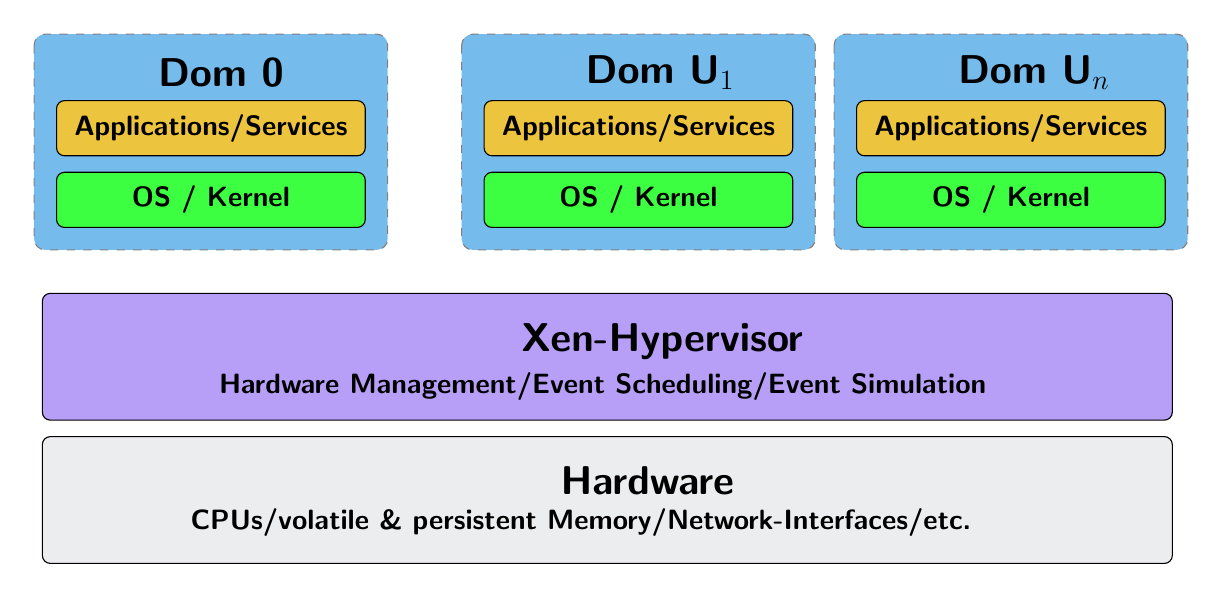
\begin{tikzpicture}[scale=0.7, every node/.style={scale=0.7},font=\sffamily,>=triangle 45]
    \tikzstyle{sum} = [draw, shape=circle, node distance=1.5cm, line width=1pt, minimum width=1.25em]    
    %\Huge
    \def\N{7}  % Number of Flip-Flops minus one
    \def\BW{1.8} % Byte Width
    
    % colors
    \definecolor{col-dom0u-app}{HTML}{E8B50C}
    \definecolor{col-dom0u-krnl}{HTML}{0DFF11}
    \definecolor{col-dom0u-bckg}{HTML}{52ABE8}
    \definecolor{col-xen-hyperv}{HTML}{4B0CE8}    
    \definecolor{col-hardware}{HTML}{CFD2D4}
    
    % dom 0
    \node (rc-dom0-app) [rectangle, fill=col-dom0u-app!80, draw, minimum width=56mm, minimum height=10mm, rounded corners=1mm] at (0,0){\Large{\textbf{Applications/Services}}};
    \node (rc-dom0-krnl) [rectangle, below= 2mm of rc-dom0-app, fill=col-dom0u-krnl!80, draw, minimum width=56mm, minimum height=10mm, rounded corners=1mm] {\Large{\textbf{OS / Kernel}}};
    \begin{pgfonlayer}{background}    
    \path (rc-dom0-app.west |- rc-dom0-app.north)+(-0.4,1.2) node (dom0-nw) {};
    \path (rc-dom0-krnl.east |- rc-dom0-krnl.south)+(0.4,-0.4) node (dom0-se) {};
    \path [fill=col-dom0u-bckg!80,rounded corners, draw=black!50, dashed] (dom0-nw) rectangle (dom0-se); 
    \node[black, below right=4mm and 14mm of dom0-nw, anchor=west] (lbl-dom0) {\huge{\textbf{Dom 0}}};    
    \end{pgfonlayer}
    
    % dom U 1
    \node (rc-domu1-app) [rectangle, right=15mm of rc-dom0-app.east, fill=col-dom0u-app!80, draw, minimum width=56mm, minimum height=10mm, rounded corners=1mm]{\Large{\textbf{Applications/Services}}};
    \node (rc-domu1-krnl) [rectangle, below= 2mm of rc-domu1-app, fill=col-dom0u-krnl!80, draw, minimum width=56mm, minimum height=10mm, rounded corners=1mm] {\Large{\textbf{OS / Kernel}}};
    \begin{pgfonlayer}{background}    
    \path (rc-domu1-app.west |- rc-domu1-app.north)+(-0.4,1.2) node (domu1-nw) {};
    \path (rc-domu1-krnl.east |- rc-domu1-krnl.south)+(0.4,-0.4) node (domu1-se) {};
    \path [fill=col-dom0u-bckg!80,rounded corners, draw=black!50, dashed] (domu1-nw) rectangle (domu1-se); 
    \node[black, below right=4mm and 14mm of domu1-nw, anchor=west] (lbl-dom0) {\huge{\textbf{Dom U$_1$}}};    
    \end{pgfonlayer}    
    
    % dom U n
    \node (rc-domun-app) [rectangle, right=8mm of rc-domu1-app.east, fill=col-dom0u-app!80, draw, minimum width=56mm, minimum height=10mm, rounded corners=1mm]{\Large{\textbf{Applications/Services}}};
    \node (rc-domun-krnl) [rectangle, below= 2mm of rc-domun-app, fill=col-dom0u-krnl!80, draw, minimum width=56mm, minimum height=10mm, rounded corners=1mm] {\Large{\textbf{OS / Kernel}}};
    \begin{pgfonlayer}{background}    
    \path (rc-domun-app.west |- rc-domun-app.north)+(-0.4,1.2) node (domun-nw) {};
    \path (rc-domun-krnl.east |- rc-domun-krnl.south)+(0.4,-0.4) node (domun-se) {};
    \path [fill=col-dom0u-bckg!80,rounded corners, draw=black!50, dashed] (domun-nw) rectangle (domun-se); 
    \node[black, below right=4mm and 14mm of domun-nw, anchor=west] (lbl-dom0) {\huge{\textbf{Dom U$_n$}}};    
    \end{pgfonlayer}    
    
    % Xen-Hypervisor
    \node (rc-xen-hyperv) [rectangle, below right = 32mm and 1mm of dom0-nw.south, fill=col-xen-hyperv!40, draw, minimum width=205mm, minimum height=23mm, rounded corners=1mm]{};    
    \node[black, below right=3mm and 60mm of rc-xen-hyperv.north west] (lbl-xen-hyperv) {\huge{\textbf{Xen-Hypervisor}}};
    \node[black, below left=0mm and -42mm of lbl-xen-hyperv.south] (lbl-xen-hyperv-detail) {\Large{\textbf{Hardware Management/Event Scheduling/Event Simulation}}};
    
    % Hardware
    \node (rc-hardware) [rectangle, below right = 2mm and 0mm of rc-xen-hyperv.south west, fill=col-hardware!40, draw, minimum width=205mm, minimum height=23mm, rounded corners=1mm]{};    
    \node[black, below right=3mm and 65mm of rc-hardware.north west] (lbl-hardware) {\huge{\textbf{Hardware}}};
    \node[black, below left=0mm and -42mm of lbl-hardware.south] (lbl-hardware-detail) {\Large{\textbf{CPUs/volatile \& persistent Memory/Network-Interfaces/etc. }}};    
    
    %    \draw [->] (jiff0.south) -- (xjlch0.north);    
    %    \draw [->,black, line width=2pt] (rc-dom0-app.east)+(0.5,0.0) -- (rc-dom0-app.east)+(0.0,0.0);
    \end{tikzpicture}   
	\caption{Xen Architecture} \label{fig:xen-arch}
\end{figure}


\subsection{Xen-Hypervisor}
The Xen-Hypervisor is a lightweight software layer (<150,000 lines of code \cite{xenprjct}) managing any kind of ressource access between virtual machines and system hardware. Thinking in a layered architecture, it is located between the hardware and the environment of virtual machine instances, so called domains. This seup is achived by a modified behaviour in the boot loader logic. Instead of loading an operating system kernel, the Xen-Hypervisor is bootstraped at first. When initialized, Xen starts loading a priviliged virtual machine, the Domain 0 (Dom 0)
which is dedicated to administer further non-priviliged virtual machines, so called Domain U{\small \textit{s}} (Dom U).

\subsection{Domain 0}\label{sub:dom0}
In the Xen-Architecture, Domain 0 is a virtual machine having special privileges. As illustarted in \ref{fig:xen-arch} Dom 0 is a meditaor between Domain U instances and the hypervisor. Since it is required for any adminstrative tasks, it is automatically started with and by the hypervisor. To manage and configure Domain U instances, a control stack, also called Toolstack, is integrated in Domain 0. To accomplish adminstrative tasks, a commandline- and graphical interface is available. For frameworks like \gls{openstck} an additional cloud orchestration stack can be added.

\subsection{Domain U}\label{sub:domu}
Domain U is the Xen terminilogy for the actual virtual machine instances provided to clients to host their applications or services. The lifecycle i.e. state of a Dom U is managed by Dom 0 (see \ref{sub:dom0}). Physically a Dom U constist of one or more images, depending on operating system. Those must be accessible to Domain 0. For the experimenatl setup of this thesis the Dom U images where stored in Dom 0 filesystem. Another approach is to keep the Dom U physical representation in an own partition on Dom 0. To mention again, a Domain is a virtual environemnt in which a virtualized operation system is running. This environment is described via a parameters per Dom U, usually persisted in configuration files accessible to Dom 0. Each Domain U can have i.e. be transfered to a certain state, controlled via commands provided by the toolstack (see \cite{xenxl}). As far as applied in the setup for this theisis, those will be described in the following.

\begin{itemize}
	\item \textbf{create (command)} Create a new virtual enviroment to bring up a virtual machine instance. All parameters required to initialize the environment are passed. Per default, the configured operating system image would be booted automatically within the created Domain. Though, a switch allowes set Domain in state Pause, i.e. to interrupt the startup process after the new Domain has been allocated, but before the virtual machine 'is powered on'. At this point, various runtime parameters can be set, f.e. BIOS serial number, BIOS vendor ID etc.
	\item \textbf{unpause (command)} Resume execution of a Domain which has previously been set to state paused.
	\item \textbf{destroy (command)} This command terminates the Domain quite radicaly. The virtualized operating system is given no chance for any shut-down procedure etc. The effect of destroy can be compared to the one pulling the plug has on an opertaing system installed on a physicaly machine \cite{xenxl}.
\end{itemize}

\section{Virtualization Modes}
In generall, code beeing run by an operrating system is executed in \gls{usrmd} or \gls{knlmd}. During the runtime of an application or service, countless switches between both modes occure. An ftp server in general is running in usermode. However, to communicate a network-interface, the needs to use a device driver which is running in kernel mode. User and kernel mode vary in their priviliges regarding the access to hardware ressources. While code running in kernel mode is allowed to access any ressource at any time, priviliges within the boundaries of user mode are restricted to f.e. a certain memory range. The motivation for this concept is an increase in system stability and security since not every application can 'do whatever it wants'. The x86 plattform enables seperate privileged modes by a hardware implementation of a ring-concept \cite{guide2017intel}.\\
A fundamental challenge in the developement of a hypervisor is how kernel mode operations of virtual guests (Dom U{\small \textit{s}}) are handled. The creation of a new domain (which requires \gls{root} priviliges) starts a process in user mode. Thus any kernel mode operation conducted by a Domain U would crash immediately. The Xen hypervisor offers several solutions which address this issue. Two important concepts will be presented in the following.  

\subsection{Paravirtualization (PV)}\label{sub:pv}
On paravirtualized operating system, a call requiring higher priviliges is delegated via a special interface through Domain 0 to the hypervisor. This presupposes, that the Dom U kernel implements this interface i.e. uses corresponding device drivers. Depending on the operating system running as guest this approach is not an option. Compared to other virtualization modes the caused overhead comapred to an on hardware installed operating system is quite reasonable \cite{xenprjct}.

\subsection{Hardware Virtual Machine (HVM)}\label{sub:hvm}
This concept, also known as hardware-assisted virtualization, enables full virtualization. In other words, no further modification of the guest operating system is required. Thus, also proprietary systems, lacking implementations supporting PV, can be virtualized. In HVM mode, critical calls of the guest, requiring higher priviliges, are translated into instructions belonging to a special instruction set, dedicated to support hardware-assisted virtualization. Intel$^\text{\textregistered}$ labeled these Virtual Machine Extensions 'Intel VT-x'. Performance of virtual machines running in HVM mode depends on the applied guest operating system \cite{xenprjct}.  


\section{Dom U Configuration}
The creation of a Domain U instance can be configured by a variety of parameters (see \cite{xenxl}). Commonly 
those are passed to the create command via configuration file. In the following the settings relevant for this thesis i.e. deviating from default will be described.

\begin{itemize}
	\item \textbf{builder} The domain build function
	\item \textbf{nr\_cpus} twezrtwezr 
	
	builder='hvm'
	
	\item \textbf{Time Stamp Counter Mode [\textsf{tsc\_mode}]} The x86 "timestamp counter", or TSC, is a 64-bit register on each processor that increases monotonically \cite{xentscmode} (TSC is further explained in \ref{itm:cycles-counter}). The current value of the register can be retrieved via the \textsf{RDTSC} instruction. Depending on the required accuracy, \textsf{tsc\_mode} can be set to one of the following values:
	\begin{itemize}
		\item \textit{always emulate} All \textsf{RDTSC} instructions are emulated. Recommended for TSC-sensitive applications at the price of a performance overhead \cite{xentscmode}.
		\item \textit{never emulate} If applications are TSC-resilient can be choosen. This mode offers best performance.
		\item \textit{Paravirtualized TSC} To achive high accuracy at high performance a hybrid mode can be applied. This requires a modification of TSC-sensitiv applications.
	\end{itemize}
\end{itemize}

% xenstore-write /bios-strings/system-manufacturer
% xenstore-write /bios-strings/system-serial-number 

\section{Virtual Machine States and Startups}
Compared to an operating system classicly installed on hardware, virtual machines can be brought up in serveral ways. Depending on the purpose i.e. the requirements of applications and services regarding availability and persistability one of the following virtual machine startup models may be applied:

\begin{itemize}
	\item \textbf{Statefull Startup} The system is started and shut down traditionally. With the shutdown the system's filesystem state is persisted. Applications and services are signaled to run termination procedures to ensure data integrity if required. With the next system start, this state will be the baseline. This startup model may be applied if f.e. database systems (i.e. database files) are hosted.
	\item \textbf{Fixed Image Startup} For a scenario not requiring any state persistence this model may be applied. With each startup, a fixed image having the same baseline is brought up. This approach makes sense if a service like a proxy-sever is hosted (log files etc. may be kept on a remote machine). For a provider this practice has a major advantage regarding maintainability. Even for a large number of clients a single fixed image may be sufficient. This simplifies f.e. provision of up to date versions and is the default of Amazons EC2 TODOP gls{IaaS} systems \cite{everspaugh2014not}.
	\item \textbf{Snapshot Startup} As mentioned in \ref{sub:domu} a Xen Domain U can be paused. If a running virtual machine is transfered to pause state, a snapshot of the entire system state is persisted. This includes filesystem, memory content, cpu registeres etc. When a machine is unpaused this state is resumed.	
\end{itemize}
%------------------------------------sdfasfd
%\cite{everspaugh2014not}
%Second,aVM  can be repeatedly executed froma ?xed image which is the default for amazon
%Dort auch: infos zu regualr boot/snapshot/masterimage
%------------------------------------
%
%Xen Domu KOnfiguration erwahnen, zB. Anzahl an CPUS
%
%However, while there are many reasons to utilize virtual machines, most of the standard security practices of operating systems are based on assumptions that hold true for physical machines, but don't translate immediately into the domain of virtualized machines \cite{kerrigan2012study}. A virtual hosted Linux server f.e. will never receive a user triggered event during the boot process, which is a critical period within the initialization of the internal Linux PRNG. Further, new virtual machine instances are usually provided by cloning a master image, instead of running an installation setup, leading to a higher degree of homogeneity among virtual machine instances. While provisioning time and maintenance benefit from this practice, it may be regarded critical. If this approach f.e. is applied as the standard process of a cloud hosting provider, it`s customers may be delivered a vulnerable system from the outset, since one customer might gain insights regarding another customers system, just by analyzing his own. These insights can be used to exploit VM reset vulnerabilities which take advantage of the reuse of  operating system snapshots, so called snapshot replay. Thomas Ristenpart et. al. describe this type of attack and apply it on TSL implementations with disastrous results. Relevant reasons they identified are the exposure of randomness, as well as the inability to find sufficient entropy in virtual systems environments \cite{ristenpart2010good, ristenpart2009hey}. \\~\\
%According to a study of Gartner from 2016, the market for x86 server virtualization infrastructure software is partitioned among few competitors, led by VMWare, Microsoft, Oracle and Red Hat. While VMWare and Microsoft offer proprietary solutions, Oracle and Red Hat adopted the open-source Xen-hypervisor technology. For cloud infrastructures, the Xen-hypervisor remains the most widely used architecture for public infrastructure as a service (IaaS) cloud provider. This fact is predominantly attributable to Amazon's utilization of the Xen-hypervisor for its cloud solutions "Amazon Web Services" \cite{bittman2016magic}. 
%
%Similarly, the market of common server operating systems can be divided into proprietary and open-source solutions. While Microsoft dominates the fraction of proprietary systems with its Windows Server series, Linux based systems have a total share of \~37\%. Within this share, \~39\% of servers dedicated to host websites etc. are running an Ubuntu Distribution \cite{statsharelinux} . \\~\\




%%The non-default choices for tsc_mode are:
%%- tsc_mode=1 (always emulate). All rdtsc instructions are emulated;
%%this is the best choice when TSC-sensitive apps are running and
%%it is necessary to understand worst-case performance degradation
%%for a specific hardware environment.
%%- tsc_mode=2 (never emulate).  This is the same as prior to Xen 4.0
%%and is the best choice if it is certain that all apps running in
%%this VM are TSC-resilient and highest performance is required.
%%- tsc_mode=3 (PVRDTSCP).  High-TSC-frequency apps may be paravirtualized
%%(modified) to obtain both correctness and highest performance; any
%%unmodified apps must be TSC-resilient.
%
%
%
%The x86 "timestamp counter", or TSC, is a 64-bit register on each
%processor that increases monotonically.  Historically, TSC incremented
%every processor cycle, but on recent processors, it increases
%at a constant rate even if the processor changes frequency (for example,
%to reduce processor power usage).  TSC is known by x86 programmers
%as the fastest, highest-precision measurement of the passage of time
%so it is often used as a foundation for performance monitoring.
%And since it is guaranteed to be monotonically increasing and, at
%64 bits, is guaranteed to not wraparound within 10 years, it is
%sometimes used as a random number or a unique sequence identifier,
%such as to stamp transactions so they can be replayed in a specific
%order
%\cite{xentscmode}


% ... and so on until
\include{chap-n}
\chapter{Notes}
\label{cha:notes}

\section{Experimental Setup/Analysis}
Processing/Algorithm is well known, reliance on pure hardware-events input.
------------

\section{Related Research}
 Related Research: 
 ------------------------
 As a noticeable result, Fan et al. [5]
 have proposed a corrected method to construct the statistical
 value for runs distribution test. They have shown that there
 exist some inaccuracies in the runs distribution test of NIST
 SP 800-22, and the degrees of freedom of the test statistic
 is adjusted. 
  \cite{kangadditional}
------------------------------
 Sehr aehnlicher ansatz, tracken von cycles, allerings sehr viel einfachere Bewertung 
 \cite{yoo2017analysis}

\section{NIST}


%%% Local Variables: 
%%% mode: latex
%%% TeX-master: "thesis"
%%% End: 

% NIST
---------------------------------------------------------
% https://github.com/usnistgov/SP800-90B_EntropyAssessment
 Number od reuiqred Samples 19 / 11 \cite{turan2018nist} 
The submitter makes an IID claim on the noise source, based on the submitter?s analysis of the design. The submitter shall provide rationale for the IID claim. \cite{turan2018nist} -> Auf MD5 verweisen
% SP 800-90B Introduction
 The test suite of SP 800-90B is divided into two major steps. The first step is to determine the track, IID(independent and identically distributed) or Non-IID, and the second step is to estimate the entropy of the given source. The permutation tests and additional chi-square tests are used \cite{kangadditional}
These statistical tests are conducted under the null hypothesis that the
given sample sequence of the PRNG?s output is independent
and identically distributed with the uniform distribution.
 \cite{kangadditional}


Hamano and Kaneko [6] have shown that the
overlapping template matching test included in the NIST SP
800-22 randomness test suite uses the inaccurate occurrence
probabilities of the template.
 \cite{kangadditional} direkete Quelle bereits bekannt
In this paper, we concentrate on the additional chi-square tests and analyze them from the view point of the nonparametric
 statistical method \cite{kangadditional}
The experimental results show that the additional chi-square tests with the corrected degrees of freedom are more effective. \cite{kangadditional}
 Since we cannot obtain an appopriate hypothesis about the distribution of the noise source which is a component of the entropy source model, assume the distribution of the entropy source is unknown. \cite{kangadditional}




\section{Discussion}

'It has been shown that the overlapping template matching test included in the NIST randomness test suite uses the inaccurate occurrence probabilities PI of the template.'
\cite{hamano2007correction,chen2016templates}. \cite{chen2016templates} proposal of approach, identification of relevant templates by correlation check. If templates B \&  B' have low correlation
both are selected for a test. If the correlation is high just one of both is chosen, as it is assumed to represent the discarded to the greatest extent. This approach reduces the amount of templates significantly (50 \%) \cite{chen2016templates}.

------------

BIOS serial number is ignored

------------

cycles and jiffies may provide more entropy at ungleichermassiger CPU load

------------

interrupt analyse ocnfidence lvele 0.05 ausreichend ?

------------
zu geringe timing variazen die dazu fuehren dass hardware vents nicht verabreitet werden bleiben unberuecksichtigt
------------

 Wenn mehr samples entnommen als bis KEETYPERANDOMINTECRETSET eintritt (wegen Number od reuiqred Samples) darauf hinweisen.
 
 ------------------------
 nicht nachvollziehbar:
  The entropy sources use emulated hardware in the guest. In cloud systems, the only source of entropy(100%) is disk \cite{kumari2015analysis}
 @phdthesis{kumari2015analysis,
     title={Analysis of Linux Random Number Generator in Virtualized Environment},
     author={Kumari, Rashmi},
     year={2015},
     school={University of Calgary}
 }
 

\include{conclusion}

% If you have appendices:
\appendixpage*          % if wanted
\appendix
\chapter{The First Appendix}
\label{app:A}

\lstinputlisting[caption=Declaration of function add\_interrupt\_randomness in Linux kernel 4.4 \cite{kernlrandmc}, captionpos=b, label=lst:add-interrupt-randomnes-c]{add-interrupt-randomnes.c}



\section{More Lorem}
\lipsum[50]

\subsection{Lorem 15--17}
\lipsum[15-17]

\subsection{Lorem 18--19}
\lipsum[18-19]

\section{Lorem 51}
\lipsum[51]

%%% Local Variables: 
%%% mode: latex
%%% TeX-master: "thesis"
%%% End: 

% ... and so on until
\include{app-n}

\backmatter
% The bibliography comes after the appendices.
% You can replace the standard "abbrv" bibliography style by another one.
\bibliographystyle{abbrv}
\bibliography{references}

\end{document}

%%% Local Variables: 
%%% mode: latex
%%% TeX-master: t
%%% End: 
